\section{Appendix: Protocol, Architecture, and Supplementary Analyses}
\label{app:main}

This appendix supports replication of the scientific protocol and visualizes module interactions.
Software-engineering artifacts are omitted.

\subsection{Experimental configuration}

Table~\ref{tab:app_config} lists core configuration values shared by both climate-risk societies.

\begin{table}[h]
\centering
\caption{Shared configuration for the two full-protocol replications.}
\label{tab:app_config}
\small
\begin{tabular}{@{}lp{0.55\textwidth}@{}}
\toprule
Parameter & Value \\
\midrule
Population & 26 agents (12 developed, 14 developing) \\
Horizon & 30 rounds \\
Institutional assignment & Forced: developed $\to$ SI; developing $\to$ SFI \\
Public-good multiplier $m$ & 1.6 \\
Stage-1 budget & Current wealth (non-negative) \\
Stage-2 budget (SI) & $\max(20,\lfloor 0.05\times\mathrm{wealth}\rfloor)$ \\
Punishment effect / cost (default) & 3 / 1 \\
Reward effect / cost & 1 / 1 \\
Initial subsidy fraction & 0.20 of punishment costs to top contributors \\
Shock schedule & Round 5 severity 0.10; round 10 severity 0.20 \\
Vulnerability & Developed 0.30; developing 1.50 \\
Damage scale factor & $150000 \times$ severity $\times$ vulnerability \\
LDF deposit rule & Stage-1 contribution dual-use deposit each round \\
LDF recipients & Developing agents after shocks \\
Initial max coverage & 0.90 \\
Initial equity weight & 0.00 (democratically revisable) \\
Democracy interval & Every 5 rounds \\
Consistency / gossip & Enabled; bulletin if score $\le 7$; max 5 items \\
Decision model & Meta Llama 3.1 8B \\
Default sampling & temperature $0.5$, $\mathrm{top}\_p=0.95$ \\
ToM / democracy temps & $0.3$ / proposal $0.5$, vote $0.3$ \\
Context length & 4096 tokens \\
Independent replications & Two random seeds (Run~A, Run~B) \\
\bottomrule
\end{tabular}
\end{table}

\subsection{Round protocol}

Each round proceeds as follows.
\begin{enumerate}
\item Institutional assignment is applied.
\item Agents choose Stage-1 contributions under decision cards, climate role guidance, beliefs, and any gossip bulletins.
\item Stage-1 public-good returns are distributed within each institution.
\item Dual-use deposits update the loss-and-damage pool.
\item SI agents allocate Stage-2 punishments and rewards.
\item Pairwise consistency scoring updates peer judgments and aggregate reputation.
\item Eligible low scores generate gossip bulletins for later rounds.
\item If the round index is divisible by five, agents propose and vote on whitelist parameters.
\item If the round is a shock round, damages and developing-country payouts are realized.
\item Wealth, beliefs, and histories update for the next round.
\end{enumerate}

\subsection{Architecture: module interaction map}

Figure~\ref{fig:app_pipeline} shows the intra-round control flow.
Figure~\ref{fig:app_feedback} shows cross-round information feedback into the next contribution prompt.
Figure~\ref{fig:app_semantic} distinguishes architectural writes from semantic reads, including the hidden loss-and-damage pool balance.
Figure~\ref{fig:app_dualuse} isolates the dual-use Stage-1 contribution.

\begin{figure}[h]
\centering
\begin{tikzpicture}[
  font=\scriptsize,
  box/.style={draw, rounded corners=2pt, align=center, inner sep=3pt, minimum width=2.1cm},
  arr/.style={-{Latex}, thick}
]
\node[box] (start) {Round start};
\node[box, right=0.35cm of start] (inst) {Institution\\assignment};
\node[box, right=0.35cm of inst] (c1) {Stage-1\\contributions};
\node[box, right=0.35cm of c1] (pg) {Public-goods\\distribution};
\node[box, below=0.55cm of pg] (s2) {Stage-2\\SI sanctions};
\node[box, left=0.35cm of s2] (sub) {Subsidy\\redistribution};
\node[box, left=0.35cm of sub] (shock) {Shock \&\\LDF payouts};
\node[box, left=0.35cm of shock] (pay) {Wealth\\update};
\node[box, below=0.55cm of pay] (rec) {History \&\\beliefs};
\node[box, right=0.35cm of rec] (tom) {Pairwise\\scoring};
\node[box, right=0.35cm of tom] (gos) {Gossip\\bulletin};
\node[box, right=0.35cm of gos] (demo) {Democracy\\if interval};
\node[box, below=0.55cm of demo] (end) {Round end};
\draw[arr] (start) -- (inst);
\draw[arr] (inst) -- (c1);
\draw[arr] (c1) -- (pg);
\draw[arr] (pg) -- (s2);
\draw[arr] (s2) -- (sub);
\draw[arr] (sub) -- (shock);
\draw[arr] (shock) -- (pay);
\draw[arr] (pay) -- (rec);
\draw[arr] (rec) -- (tom);
\draw[arr] (tom) -- (gos);
\draw[arr] (gos) -- (demo);
\draw[arr] (demo) -- (end);
\end{tikzpicture}
\caption{Intra-round module pipeline.
Democracy applies only on interval rounds; otherwise the society proceeds directly to round end.}
\label{fig:app_pipeline}
\end{figure}

\begin{figure}[h]
\centering
\begin{tikzpicture}[
  font=\scriptsize,
  box/.style={draw, rounded corners=2pt, align=center, inner sep=3pt},
  arr/.style={-{Latex}, thick}
]
\node[box] (act) {Actions$_t$};
\node[box, right=1.1cm of act] (pay) {Payoffs /\\wealth$_t$};
\node[box, right=1.1cm of pay] (tom) {Scores$_t$};
\node[box, below=0.7cm of tom] (rep) {Reputation$_t$};
\node[box, left=1.1cm of rep] (gos) {Gossip$_t$};
\node[box, left=1.1cm of gos] (bel) {Beliefs$_t$};
\node[box, below=0.7cm of bel] (pr) {Prompts$_{t+1}$};
\node[box, right=2.4cm of pr] (act2) {Actions$_{t+1}$};
\draw[arr] (act) -- (pay);
\draw[arr] (act) -- (tom);
\draw[arr] (pay) -- (bel);
\draw[arr] (tom) -- (rep);
\draw[arr] (tom) -- (gos);
\draw[arr] (bel) -- (pr);
\draw[arr] (rep) -- (pr);
\draw[arr] (gos) -- (pr);
\draw[arr] (pr) -- (act2);
\end{tikzpicture}
\caption{Cross-round feedback.
Reputation and gossip from round $t$ enter prompts in round $t+1$.
The numeric loss-and-damage pool balance is not fed into prompts.}
\label{fig:app_feedback}
\end{figure}

\begin{figure}[h]
\centering
\begin{tikzpicture}[
  font=\scriptsize,
  box/.style={draw, rounded corners=2pt, align=center, inner sep=3pt, minimum width=1.7cm},
  dashbox/.style={draw, dashed, rounded corners=2pt, align=center, inner sep=3pt, minimum width=1.7cm},
  arr/.style={-{Latex}, thick},
  darr/.style={-{Latex}, thick, dashed}
]
\node[box] (c) {Stage-1\\contribution};
\node[box, above right=0.4cm and 1.2cm of c] (tom) {Pairwise\\scores};
\node[box, right=2.6cm of tom] (rep) {Reputation};
\node[box, below=0.9cm of rep] (gos) {Gossip};
\node[box, below=0.9cm of c] (s2) {Stage-2\\(SI)};
\node[box, right=1.4cm of s2] (bel) {Belief\\labels};
\node[dashbox, left=1.2cm of c] (pool) {LDF pool\\(hidden)};
\node[box, below left=0.5cm and 0.2cm of pool] (own) {Own payout\\/ damage};
\node[box, below=1.6cm of bel] (next) {Next contribution\\prompt};
\node[box, right=1.6cm of next] (demo) {Democracy\\parameters};
\draw[arr] (c) -- (tom);
\draw[arr] (tom) -- (rep);
\draw[arr] (tom) -- (gos);
\draw[arr] (c) -- (s2);
\draw[arr] (c) -- (bel);
\draw[arr] (c) -- (pool);
\draw[darr] (pool) -- node[above, font=\tiny]{not observed} (next);
\draw[arr] (rep) -- (next);
\draw[arr] (gos) -- (next);
\draw[arr] (s2) -- (next);
\draw[arr] (bel) -- (next);
\draw[arr] (own) -- (next);
\draw[arr] (demo) -- (next);
\end{tikzpicture}
\caption{Semantic coupling among modules.
Solid arrows are information channels available to agents.
The dashed edge marks an architectural write without a semantic read: the live pool balance is hidden.}
\label{fig:app_semantic}
\end{figure}

\begin{figure}[h]
\centering
\begin{tikzpicture}[
  font=\scriptsize,
  box/.style={draw, rounded corners=2pt, align=center, inner sep=4pt},
  arr/.style={-{Latex}, thick}
]
\node[box] (c) {Stage-1 contribution $c_i$};
\node[box, above right=0.55cm and 1.4cm of c] (pg) {Institution\\public-good share};
\node[box, below right=0.55cm and 1.4cm of c] (ldf) {LDF pool\\deposit};
\draw[arr] (c) -- (pg);
\draw[arr] (c) -- (ldf);
\end{tikzpicture}
\caption{Dual-use Stage-1 contribution.
One decision funds both institutional public-good returns and the loss-and-damage pool.}
\label{fig:app_dualuse}
\end{figure}

Canonical narrative flow for an agent is:
observation $\rightarrow$ reasoning $\rightarrow$ contribution $\rightarrow$ reputation $\rightarrow$ gossip $\rightarrow$ proposal $\rightarrow$ vote $\rightarrow$ parameter change $\rightarrow$ later contribution.
In climate mode, democratic ``institutional change'' means parameter change, not free switching between SI and SFI.

\subsection{Prompt templates (sanitized)}

\subsubsection{Default behavioral persona}

\begin{quote}
\small
Act in whatever way maximizes your own cumulative payoff over the game.
Cooperation, free-riding, punishment, or defection are all valid if they serve your interests.
Do not assume you have any obligation to the group.
Treat other agents as strategic variables.
Use past rounds to identify patterns you can exploit or respond to.
Keep choices valid under all game rules and cite the concrete facts driving your decision.
\end{quote}

\subsubsection{Climate role guidance}

\begin{quote}
\small
\textbf{Developed country.}
You typically have higher fiscal capacity and historically higher emissions.
Treat long-run climate stability and institutional credibility as strategically important.
You are assigned to the binding treaty institution with peer sanctioning.

\textbf{Developing country.}
You typically face higher climate vulnerability and tighter fiscal constraints.
Treat disaster compensation and survival constraints as strategically important.
You are assigned to the non-binding agreement without peer sanctioning.
\end{quote}

\subsubsection{Stage-1 contribution decision}

\begin{quote}
\small
Choose an integer contribution between 0 and your current budget.
You observe group size, marginal per-capita return, recent same-institution averages, own wealth, beliefs, and any gossip bulletins.
State a brief rationale for the chosen amount.
\end{quote}

\subsubsection{Stage-2 sanction decision (SI only)}

\begin{quote}
\small
Allocate your sanction budget across listed peers as punishments and rewards.
Punishments and rewards must be non-negative integers that respect the budget.
Provide a brief justification that is consistent with the numeric allocation.
\end{quote}

\subsubsection{Pairwise consistency scoring}

\begin{quote}
\small
Score the target from 1 to 10 for consistency between stated intent and observed action.
Provide a one-sentence justification.
Low scores may generate gossip bulletins.
\end{quote}

\subsubsection{Democracy proposal and vote}

\begin{quote}
\small
Propose at most one whitelist parameter change, or abstain.
Later, vote yes or no on each eligible proposal.
Whitelist items include subsidy fraction, subsidy breadth, punishment effect, reward effect, and loss-and-damage equity or damage weights.
\end{quote}

\subsection{Supplementary statistics}

Table~\ref{tab:app_cross_corr} reports cross-replication correlations of round-mean intensity.
Table~\ref{tab:app_shock} reports Wilcoxon tests around shock rounds.
Figure~\ref{fig:app_shockbox} shows shock-delta distributions.
Figure~\ref{fig:app_agent} shows agent-mean intensity scatter across replications.

\begin{table}[h]
\centering
\caption{Cross-replication correlation of round-mean contribution intensity.}
\label{tab:app_cross_corr}
\small
\begin{tabular}{lrrr}
\toprule
Series & Pearson $r$ & $p$ & RMSE \\
\midrule
All agents & 0.194 & 0.305 & 0.124 \\
SI only & 0.144 & 0.448 & 0.164 \\
SFI only & 0.020 & 0.916 & 0.184 \\
\bottomrule
\end{tabular}
\end{table}

\begin{table}[h]
\centering
\caption{Within-agent shock event-study Wilcoxon tests for $\Delta\mathrm{prop}$.}
\label{tab:app_shock}
\small
\begin{tabular}{lccrr}
\toprule
Run & Shock & Mean $\Delta$ & Median $\Delta$ & Wilcoxon $p$ \\
\midrule
A & R5 & $+0.023$ & $-0.014$ & 0.367 \\
A & R10 & $+0.010$ & $+0.015$ & 0.328 \\
B & R5 & $-0.080$ & $-0.011$ & 0.582 \\
B & R10 & $+0.050$ & $-0.147$ & 0.367 \\
\bottomrule
\end{tabular}
\end{table}

\begin{figure}[h]
\centering
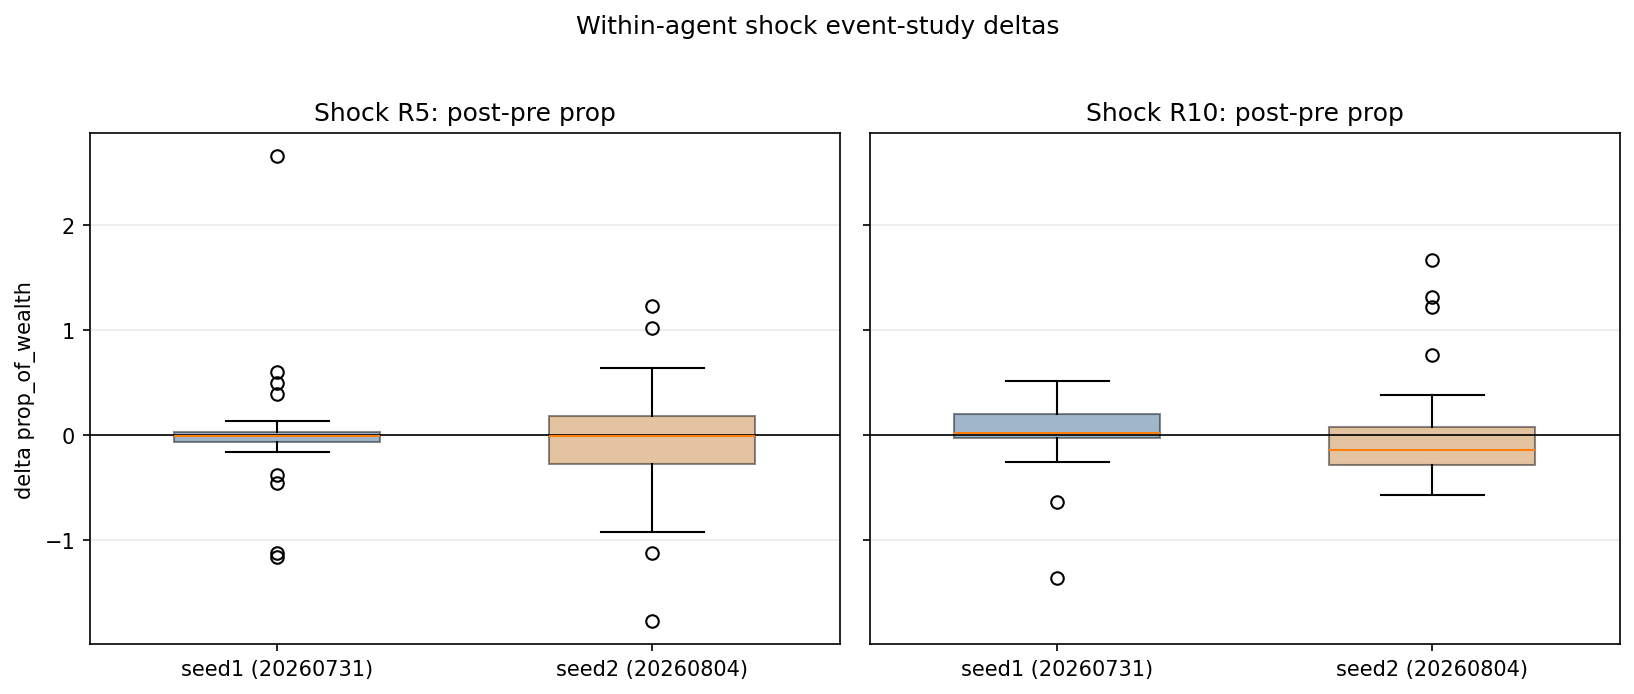
\includegraphics[width=0.72\textwidth]{figures/shock_delta_boxplot_cross_seed.png}
\caption{Within-agent post-minus-pre intensity changes around climatic shocks.}
\label{fig:app_shockbox}
\end{figure}

\begin{figure}[h]
\centering
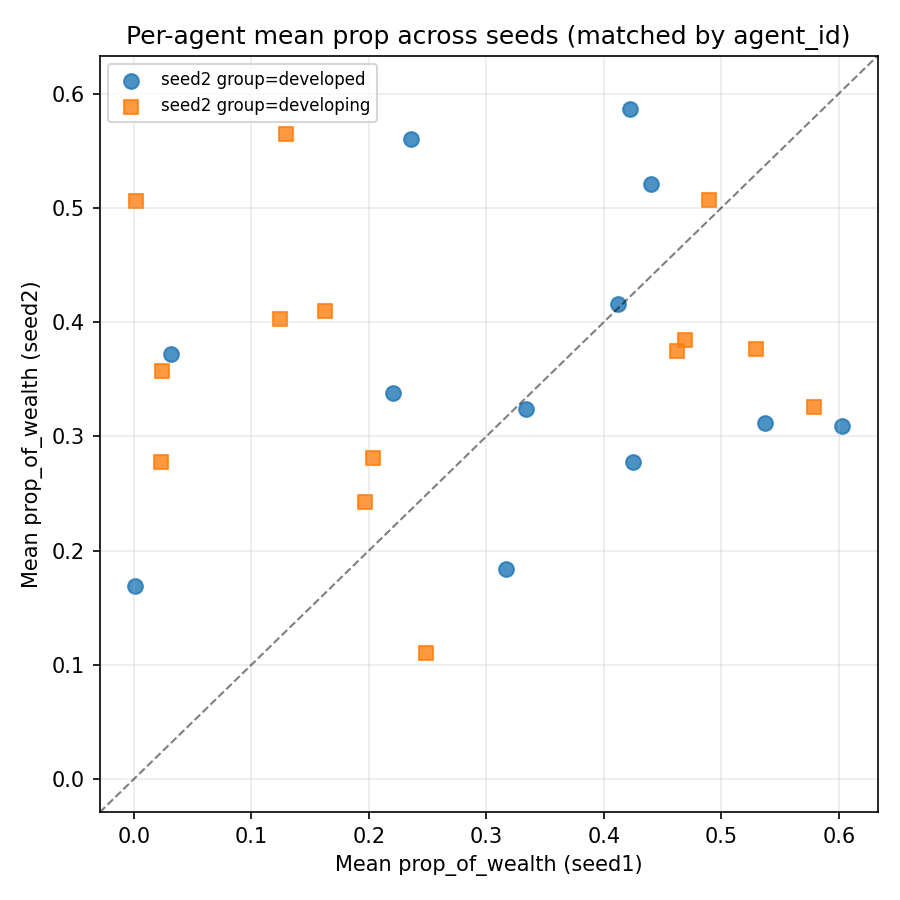
\includegraphics[width=0.72\textwidth]{figures/agent_mean_prop_scatter.png}
\caption{Agent-mean contribution intensity in Run~A versus Run~B.
Points are not persona-matched across replications.}
\label{fig:app_agent}
\end{figure}

\subsection{Motif codebook}

\begin{itemize}
\item \emph{Opportunistic:} free-riding, self-interest, payoff maximization, or marginal-return language.
\item \emph{Conformity:} peer or group-average behavior as the reason for the agent's own choice.
\item \emph{Reputation management:} explicit standing, credibility, trust scores, or avoiding a free-rider label.
\item \emph{Named agents:} reference to a specific peer identifier.
\item \emph{Future-rounds:} intertemporal conservation without a stronger primary motif.
\item \emph{Gossip reference:} explicit gossip or bulletin language.
\end{itemize}

\subsection{Claim boundaries}

Supported under the present protocol: recurring SFI withdrawal after gossip and bad reputation; within-run SI$\approx$SFI mean intensity; coverage without equalization; history-dependent democracy.
Unsupported: causal SI-versus-SFI institution effects; universal SI gossip withdrawal; evaluation of any real-world loss-and-damage fund; full implementation of Ostrom design principles; persona-stable agent identifiers across replications.
